\documentclass{article}

\usepackage[margin=1in]{geometry} 
\usepackage{amsmath,amsthm,amssymb,amsfonts, fancyhdr, color, comment, graphicx, environ,bbm}
\usepackage[dvipsnames]{xcolor}
\usepackage{subcaption}
\usepackage{mdframed}
\usepackage[shortlabels]{enumitem}
\usepackage{indentfirst}
\usepackage{hyperref}
\usepackage{placeins}
\usepackage{comment} %Comment large blocks
\usepackage{xfrac}
\usepackage{float} % To use "H" to force tables to be where wanted
\usepackage{booktabs} % Makes output from knittr:kable look better
\usepackage{parskip} %No indents for paragraphs
\usepackage[shortlabels]{enumitem} % To enumerate with letters
\hypersetup{
 colorlinks=true,
 linkcolor=blue,
 filecolor=magenta, 
 urlcolor=blue,
}
\pagestyle{fancy}
\usepackage{todonotes}

\newcommand{\E}{\mathbb{E}}
\renewcommand{\H}{\mathcal{H}}
\renewcommand{\L}{\mathcal{L}}
\newcommand{\dU}[1]{\ensuremath\frac{\partial u}{\partial #1}}
\newcommand{\dV}[1]{\ensuremath\frac{\partial v}{\partial #1}}
\newcommand{\ppx}[2]{\ensuremath\frac{\partial #1}{\partial #2}}
\newcommand{\ddx}[2]{\ensuremath\frac{d #1}{d #2}}
\newcommand{\indp}{\perp\!\!\!\perp} 

%\usepackage{mathpazo} %Dylan's fancy math bullshit that I don't want
\usepackage{microtype}
\usepackage{graphicx}
\usepackage{setspace}

%Footnote without a number
\newcommand\blfootnote[1]{%
  \renewcommand\thefootnote{}\footnote{#1}%
  \addtocounter{footnote}{-1}%
}

% Problem formatting [Alex]

\newenvironment{problem}[1]
    { \begin{mdframed}[backgroundcolor=Periwinkle!20] \textbf{(#1)} }
    {  \end{mdframed}}
% Define solution environment
\newenvironment{solution}{\textbf{Solution}\\}

%%%%%%%%%%%%%%%%%%%%%%%%%%%%%%%%%%%%%%%%%%%%%
%Fill in the appropriate information below
\lhead{Problem Set 2}
\rhead{Empirical Analysis} 
\title{Problem Set 2}
\author{Alex Weinberg \and Isaac Norwich \and Jose M. Quintero}

%%%%%%%%%%%%%%%%%%%%%%%%%%%%%%%%%%%%%%%%%%%%%
\begin{document}
\maketitle

\begin{comment}
Q3 - 3 parts - no solutions - Jose
Q4 - 1 part  - no solutions - Alex
Q5 - 1 part  - no solutions - Jose
Q8 - 5 parts - no solutions - Isaac

Q1 - 7 parts - solutions - Isaac & Jose
Q2 - 4 parts - solutions - Jose
Q6 - 1 part  - solutions - Alex
Q7 - 3 parts - solutions - Alex

Parts:
Isaac - 5
Alex
Jose

Total of 21 parts and 2 other questions

\end{comment}


Our code can be found in this GitHub respository: \url{https://github.com/jmquintero925/Metrics-III/tree/main/ps2Heckman}


%%%%%%%%%%%%%%%%%%%%%%%%%%%%%%%%%% QUESTION 1 %%%%%%%%%%%%%%%%%%%%%%%%%%%%%%%%%
\section*{Problem 1}
Answer the questions embedded in the econometric causality model handouts based on Heckman (2008).

\begin{problem}{Question 1 Slide 27}
Question: Can agents ex ante evaluate the ex post evaluation?
\end{problem}
\begin{solution}
An agent cannot ex ante evaluate the ex post evaluation, because the ex ante expectation is conditional on the agent's information set, $\mathcal{I}$, while the ex post evaluation uses known quantities.
\end{solution}


\begin{problem}{Question 2 Slide 32}
Question: How can agents identify what might have been for states they have not experienced? Consider alternative approaches.
\end{problem}
\begin{solution}
Agents can use many different forecasting methods in order to identify what might have been for states they have not experiences. For instance, they can use ex post outcomes for individuals who they deem similar to themselves -- a version of implicit matching. Or instead they may use historical data on others or even on their previous experiences. For instance, if an agent is considering a treatment that is similar to one encountered previously, they can use their subjective information set to compare the outcomes if they do or do not take up treatment this time.
\end{solution}
 
\begin{problem}{Question 3 Slide 35}
Question: What are the precise requirements for solving P3 for the PRTE?
\end{problem}
\begin{solution}
Recall that P3 is ``forecasting the impacts of interventions never historically experienced, including their impacts on well-being." To solve P3, we must have a structural model with new, never previously experienced, ingredients. For instance, we can use the Roy Model to parameterize the decision-making process of individuals. We then need data to fit to the model: observed outcomes ($Y$), characteristics that partially determine these outcomes ($X$), and also exogenous shifters of the costs involved in treatment versus control ($W$). Then we can estimate the PRTE for one policy (a specific value of $W$) versus another (a different value of $W$).
\end{solution}
 
\begin{problem}{Question 4 Slide 36}
Question: In the context of a policy of tuition reduction, under what conditions is $Y^a_0 = Y^b_0; Y^a_1 = Y^b_1$ where $Y_i^j$ denotes the present value of life cycle earnings under policy $j$ in state $i$?
\end{problem}
\begin{solution}
With regards to tuition reduction, for policy invariance to hold, we would need the potential outcomes under treatment $a$ versus treatment $b$ to be the same. If $a$ is the current setup and $b$ was free college for anyone who wishes to attend, we would need the present value of life cycle earnings to not be impacted regardless of take up of the treatment. In this case, we would need to rule out social effects including peer effects and general equilibrium effects that would impact the potential outcomes. Policy invariance seems unlikely in this setting. If college is free, then the wage premium for having a college degree would decrease and thus invariance would not hold. 
\end{solution}

\begin{problem}{Question 5 Slide 38}
Question: What is the relationship between PRTE and ITT (Intention To Treat)? Is PRTE a causal parameter?
\end{problem}
\begin{solution}
The PRTE calculates the difference in the average outcome across the whole population between to different policies. Essentially, the PRTE calculates for the effect of a change in policy accounting for endogenous selection. Thus, by design the PRTE is a causal parameter. Similarly, the ITT tries to unveil the effect of two different policies. However, this parameter does not account for sorting or other endogenous mechanisms as it assumes that the the policy is randomized across agents. 
\end{solution}


\begin{problem}{Question 6 Slide 41}
Question: Is LATE a causal parameter? How does it address P1-P3?
\end{problem}
\begin{solution}
The LATE is the causal parameter that unveils the treatment effect for the group of compliers for a given instrument. By definition, the LATE is a causal parameter. However, by design, the LATE can only address P1. Since the LATE depends on both the policy and the group of compliers for an specific policy and instrument, it is hard to extrapolate the results out of sample and thus it can hardly address P2 and P3 without additional simplifying assumption. 
\end{solution}

\newpage
%%%%%%%%%%%%%%%%%%%%%%%%%%%%%%%%%% QUESTION 2 %%%%%%%%%%%%%%%%%%%%%%%%%%%%%%%%%
\section*{Problem 2}
Answer the questions embedded in the ``Classical Discrete Choice Theory'' handout.

\begin{problem}{Question 1 Slide 17}
Prove
\end{problem}
\begin{solution}
Let $F(\varepsilon_1,...,\varepsilon_N)$ the join CDF of the idiosyncratic shocks. Then note that
\begin{align*}
    \ppx{}{\varepsilon_j}F(\varepsilon_1,...,\varepsilon_N) &= \ppx{}{\varepsilon_j} \int_{-\infty}^{\varepsilon_1}\cdots\int_{-\infty}^{\varepsilon_j}\cdots\int_{-\infty}^{\varepsilon_N} f(x_1,...,x_N)\mathrm{d}x_1\cdots\mathrm{d}x_j\cdots\mathrm{d}x_N \\
     &= \int_{-\infty}^{\varepsilon_1}\cdots\int_{-\infty}^{\varepsilon_{j-1}}\int_{-\infty}^{\varepsilon_{j+1}}\cdots\int_{-\infty}^{\varepsilon_N} f(x_1,...,\varepsilon_j,...,x_N)\mathrm{d}x_1\cdots\mathrm{d}x_{j-1}\mathrm{d}x_{j+1}\cdots\mathrm{d}x_N
\end{align*}
where the second line uses Fubini's theorem (interchange the order of integrals) and the fact for pdfs, the integral and the derivative are commutative operations. Using this fact, note that the conditional CDF can be written as 
\begin{align*}
    F(\varepsilon_1,...\varepsilon_{j-1},\varepsilon_{j+1},...,\varepsilon_N\vert\varepsilon_j) &= \frac{1}{f_{\varepsilon_j}(\varepsilon_j)} \int_{-\infty}^{\varepsilon_1}\cdots\int_{-\infty}^{\varepsilon_{j-1}}\int_{-\infty}^{\varepsilon_{j+1}}\cdots\int_{-\infty}^{\varepsilon_N} f(x_1,...,\varepsilon_j,...,x_N)\mathrm{d}x_1\cdots\mathrm{d}x_{j-1}\mathrm{d}x_{j+1}\cdots\mathrm{d}x_N \\ 
    &=\frac{1}{f_{\varepsilon_j}(\varepsilon_j)} \ppx{}{\varepsilon_j}F(\varepsilon_1,...,\varepsilon_N)
\end{align*}
Using this equation, we can prove the result by taking conditional expectations. 
\begin{align*}
\Pr\left(\varepsilon_{I}\leq v_{j}-v_{I} + \varepsilon_{j}, \quad \forall I \neq j\right)=&\E\left[\Pr\left(\varepsilon_{I}\leq v_{j}-v_{I} + \varepsilon_{j}, \forall I \neq j\Big\vert \varepsilon_{j}\right)\right]\\
%%%%%%%
&\int_{-\infty}^{\infty} F\left(v_{j}-v_{1} + \varepsilon_{1},..., v_{j}-v_{j-1} + \varepsilon_{j},\varepsilon_{j},...v_{j}-v_{N} + \varepsilon_{j}\right) f_{\varepsilon_j}\left(\varepsilon_{j}\right) d \varepsilon_{j}\\
%%%%%%%%
&\int_{-\infty}^{\infty} \frac{\partial F}{\partial \varepsilon_{j}}\left(v_{j}-v_{1} + \varepsilon_{1},..., v_{j}-v_{j-1} + \varepsilon_{j},\varepsilon_{j},...v_{j}-v_{N} + \varepsilon_{j}\right) d \varepsilon_{j}
\end{align*}
\end{solution}

\begin{problem}{Question 2 Slide 28}
Prove why introduction of identical good changes probability of riding a bus.
\end{problem}
\begin{solution}
Consider the example discuss during class. Based on Luce Model, the probability of taking bus is:
\begin{equation*}
\operatorname{Pr}(\text{Bus} \mid\{\text{Car},\text{Bus}\}, s)=\frac{e^{\theta(s)^{\prime} x_{\text{Bus}}}}{e^{\theta(s)^{\prime} x_{\text{Car}}}+e^{\theta(s)^{\prime} x_{\text{Bus}}}}
\end{equation*}
Now consider an expanded choice set with a red bus which is identical to blue bus. Then the probability of taking bus becomes:

\begin{equation*}
\operatorname{Pr}(\text{Bus} \mid\{\text{Car},\text{Bus},\text{Red Bus}\}, s)=\frac{e^{\theta(s)^{\prime} x_{\text{Bus}}}+e^{\theta(s)^{\prime} x_{\text{Red Bus}}}}{e^{\theta(s)^{\prime} x_{\text{Car}}}+e^{\theta(s)^{\prime} x_{\text{Bus}}}+e^{\theta(s)^{\prime} x_{\text{Red Bus}}}}
\end{equation*}

Since red and blue buses can be seen as perfect substitutes, we can assume that the agent obtains same utility from them, i.e. $e^{\theta(s)^{\prime} x_{\text{Bus}}}=e^{\theta(s)^{\prime} x_{\text{Red Bus}}}$. As a result,

\begin{equation*}
\operatorname{Pr}(\text{Bus}\mid\{\text{Car},\text{Bus},\text{Bus}\}, s)=\frac{2 e^{\theta(s)^{\prime} x_{\text{Bus}}}}{e^{\theta(s)^{\prime} x_{\text{Car}}}+2 e^{\theta(s)^{\prime} x_{\text{Bus}}}} \neq \operatorname{Pr}(\text{Bus} \mid\{\text{Car},\text{Bus}\}, s)
\end{equation*}
\end{solution}


\begin{problem}{Question 1 Slide 40}
Prove this
\end{problem}
\begin{solution}
In the nested logit model, let

\begin{equation*}
G\left(e^{v_{1}}, \ldots, e^{v_{J}}\right)=\sum_{m=1}^{M} a_{m}\left[\sum_{i \in B_{m}} e^{\frac{v_{i}}{1-\sigma_{m}}}\right]^{1-\sigma_{m}}
\end{equation*}

Then,

\begin{equation*}
\begin{aligned}
& p_{i}=\frac{\partial \ln G}{\partial v_{i}}=\frac{\partial \ln \left[\sum_{m=1}^{M} a_{m}\left[\sum_{i \in B_{m}} e^{\frac{v_{i}}{1-\sigma_{m}}}\right]^{1-\sigma_{m}}\right]}{\partial v_{i}} \\
& =\frac{\sum_{m=1}^{M} a_{m}\left[\sum_{i \in B_{m}} e^{\frac{v_{i}}{1-\sigma_{m}}}\right]^{-\sigma_{m}} e^{\frac{v_{i}}{1-\sigma_{m}}}}{\sum_{m=1}^{M} a_{m}\left[\sum_{i \in B_{m}} e^{\frac{v_{i}}{1-\sigma_{m}}}\right]^{1-\sigma_{m}}} \\
& =\frac{\sum_{m=1}^{M} a_{m}\left[\sum_{i \in B_{m}} e^{\frac{v_{i}}{1-\sigma_{m}}}\right]^{1-\sigma_{m}} e^{\frac{v_{i}}{1-\sigma_{m}}}\left[\sum_{i \in B_{m}} e^{\frac{v_{i}}{1-\sigma_{m}}}\right]^{-1}}{\sum_{m=1}^{M} a_{m}\left[\sum_{i \in B_{m}} e^{\frac{v_{i}}{1-\sigma_{m}}}\right]^{1-\sigma_{m}}} \\
& =\sum_{m=1}^{M} \underbrace{\left(\frac{e^{\frac{v_{i}}{1-\sigma_{m}}}}{\sum_{i \in B_{m}} e^{\frac{v_{i}}{1-\sigma_{m}}}}\right)}_{\Pr\left(i \mid B_{m}\right)} \underbrace{\left(\frac{a_{m}\left[\sum_{i \in B_{m}} e^{\frac{v_{i}}{1-\sigma_{m}}}\right]^{1-\sigma_{m}}}{\sum_{m=1}^{M} a_{m}\left[\sum_{i \in B_{m}} e^{\frac{v_{i}}{1-\sigma_{m}}}\right]^{1-\sigma_{m}}}\right)}_{\Pr\left(B_{m}\right)} \\
& =\sum_{m=1}^{M} \Pr\left(i \mid B_{m}\right) P\left(B_{m}\right)
\end{aligned}
\end{equation*}

Observe that if $\Pr\left(B_{m}\right)=1, p_{i}=\sum_{m=1}^{M} \Pr\left(i \mid B_{m}\right)=\sum_{m=1}^{M}\left(\frac{e^{\frac{v_{i}}{1-\sigma_{m}}}}{\sum_{i \in B_{m} e^{\frac{v_{i}}{1-\sigma_{m}}}}}\right)$. Thus if 
\end{solution}

\begin{problem}{Question 2 Slide 56}
Prove it can be used to identify $\sigma_{U}^{2}$ and $\sum_{\beta}$.
\end{problem}
\begin{solution}
Under some reasonable assumptions $\hat{\beta}$ is a consistent estimator of $\beta$, then

\begin{align*}
W &=Y-X \hat{\beta} \\  
&\xrightarrow{p} Y-X \E[\beta] \\ 
&=Y-X \bar{\beta} \\
&=X(\beta-\bar{\beta})+U
\end{align*}
Given that $\E[X(\beta-\bar{\beta})+U]=0$,
\begin{equation*}
\begin{aligned}
\E\left[W^{2}\right]&=\operatorname{Var}(W) \\
&\xrightarrow{p}\operatorname{Var}(X(\beta-\bar{\beta})+U)\\
&=X^{\prime} \Sigma_{\beta} X+\sigma_{U}^{2}
\end{aligned}
\end{equation*}

Thus, by regressing squared OLS residuals $W$ on a second degree polynomial of $X$ will identify both $\sigma_u^2$ and $\Sigma_\beta$. The $y$-intercept will identify $\sigma_u^2$. The square terms identify the diagonal of the matrix. Specifically, let $\hat{\beta}_{ij}$ the coefficient with $X_iX_j$. Then $\hat{\beta}_{ij}$ identifies $\Sigma_\beta(i,j)$.  
\end{solution}

\newpage

%%%%%%%%%%%%%%%%%%%%%%%%%%%%%%%%%% QUESTION 3 %%%%%%%%%%%%%%%%%%%%%%%%%%%%%%%%%
\section*{Problem 3}
 For the model $Y=X_{1} \beta_{1}+X_{2} \beta_{2}+U$,
\begin{align*}
\begin{aligned}
&E\left(U \mid X_{1}, X_{2}\right)=0 \\
&\sum_{X_{1}, X_{2}} \text { full rank, }
\end{aligned}
\end{align*}
discuss and compare the properties of the three estimators: \\
\begin{enumerate}[label=(\alph*)]
    \item OLS $\hat\beta_1$
    \item $\bar{\beta_1}$
    \item $\tilde{\beta}_1=\begin{cases}
            \hat\beta_{1}, & \text { if } t_{\hat{\beta}_{1}} \geq 2 \\ 
            \bar{\beta}_{1}, & \text{ otherwise}
        \end{cases}$
\end{enumerate}



\begin{solution}
For each of the cases
\begin{enumerate}[label=(\alph*)]
    \item $\hat\beta_1$ from OLS is consistent and unbiased. It is not necessarily efficient though as no assumptions are given on the structure of the error terms. In the absence of heteroscedasticity then the problem would satisfy Gauss-Markov hypothesis and it will have minimal variance over the class of linear unbiased estimators. For the sake of the variance argument, assume there is homoscedasticity and the variance of the errors is $\sigma^2$. Then \begin{equation*}
        \sqrt{N}\left(\hat{\beta}_1-\beta\right) \xrightarrow{d} \mathcal{N}\left(0,\frac{\sigma^2}{1-\rho^2}\right)
    \end{equation*}
    where $\rho = \text{Corr}(X_1,X_2)$. Thus, as $\rho\to1$ the variance of the estimator goes to infinity. 
    \item Consider the formula for omitted variables
    \begin{align*}
        \hat{\beta}_1 &= \frac{\cov(Y,X_1)}{\var(X_1)} \\ 
        &= \frac{\cov(X_1\beta_1+X_2\beta_2+U,X_1)}{\var(X_1)} \\ 
        &= \beta_1 + \beta_2\frac{\cov(X_1,X_2)}{\var(X_1)} \\ 
        &= \beta_1 + \beta_2g(\rho)
    \end{align*}
    where $g$ is an increasing function of the correlation. Then the properties of this estimator are going to depend on the correlation between $X_1$ and $X_2$. If $\text{Corr}(X_1,X_2)=0$ then the estimator will be both consistent and unbiased. Otherwise it will both inconsistent and biased. Finally, the distribution of $\bar{\beta}_1$\footnote{See Heckman and Pinto paper for full derivations. } is 
    \begin{equation*}
        \bar{\beta}_1 \xrightarrow{d}\mathcal{N}\left(\beta_1+\beta_2g(\rho),\sigma^2+\beta_2^2(1-\rho^2)\right)
    \end{equation*}
    Thus,, now there is a trade-off between variance and bias. As the correlation approaches 1, then bias hits its higher bound but the estimator becomes efficient. If the correlation is 0, then there is no bias but the variance increases. 
    \item This procedure is a mixture between the two last procedures but first begin by noting that 
    \begin{equation*}
        \tilde{\beta}_1\sim\begin{cases}
        \mathcal{N}\left(0,\frac{\sigma^2}{1-\rho^2}\right) &\mbox{with prob. } \Pr(t_{\hat{\beta}_1}\geq 2) \\ 
        \mathcal{N}\left(\beta_1+\beta_2g(\rho),\sigma^2+\beta_2^2(1-\rho^2)\right) &\mbox{with prob. } 1-\Pr(t_{\hat{\beta}_1}\geq 2)
        \end{cases}
    \end{equation*}
    But note that 
    \begin{equation*}
        \Pr(t_{\hat{\beta}_1}\geq 2) \longrightarrow 1-\Phi\left(2-\frac{\beta_1}{\sqrt{\frac{\sigma^2}{1-\rho^2}}} \right) 
    \end{equation*}
    Thus as $\rho\to 1$ then $\Pr(t_{\hat{\beta}_1}\geq 2)\to 1$. Thus the the higher the correlation with the omitted, chances are that the true model will be the one. 
\end{enumerate}

\end{solution}

\newpage

%%%%%%%%%%%%%%%%%%%%%%%%%%%%%%%%%% QUESTION 4 %%%%%%%%%%%%%%%%%%%%%%%%%%%%%%%%%
\section*{Problem 4}
Answer the questions embedded in the ``Hypothesis Testing: Part I'' handout.

\begin{problem}{Slide 6}
Prove that for random variable with density (absolutely continuous with
Lebesgue measure) $Z = F_X (X )$ is uniform for any $X$ given
that $F_X$ is continuous.
\end{problem}

\begin{solution}
Given any random continuous variable X, define $Z := f(X) = F_X(X)$. Because its a probability it is in the unit interval. Define $G$ as the CDF of $Z$. Assuming requisite continuity:

\begin{align*}
G(z) &= \operatorname{P}(Z\leq z) \\
        &= \operatorname{P}(f(X)\leq z) \\
        &= \operatorname{P}(X\leq f^{-1}(z)) \\
        &= f (f^{-1}(z)) \\
        &= z
\end{align*}

QED.

\end{solution}

% ---------------------
\begin{problem}{Slide 12}
In what sense does increasing sample size always lead to rejection of an hypothesis?
\end{problem}

To fix ideas, suppose we are considering the null hypothesis that the mean is zero $H_0: \mu_0 = 0$.

If we increase the sample size by letting $T\rightarrow \infty$ then the power of our test will correspondingly go to $1$.

We reject the null if 

$$
|\bar{X}-\mu|>c(\alpha)=\frac{\sigma}{\sqrt{T}} \Phi^{-1}(\alpha)
$$

This is mechanically increasing in T. If $T$ gets large enough we will reject with probability one. However is this is kind of weird. What if the true value of the mean is $\epsilon$ infinitesimally small. It seems weird to reject in this instance. 
 

% ---------------------
\begin{problem}{Slide 29}
Verify that 75\% of the time C (X1, X2) contains $\theta_0$ (75\% of repeated trials it covers $\theta_0$). (Verify this)
\end{problem}

There are two independent draws $i=1,2$.

$$
X_{i} \sim^{iid} \begin{cases}\theta_{0}+1 & \text { prob 1/2 } \\ \theta_{0}-1 & \text { prob } 1 / 2\end{cases}
$$
Then, for two draws, the probability that both draws are the same is $1 / 2$, and the probability that the draws are different is $1 / 2$. 

The confidence interval from the question is:
 
$$
C\left(X_{1}, X_{2}\right)= \begin{cases}\frac{1}{2}\left(X_{1}+X_{2}\right) & \text { if } X_{1} \neq X_{2} \\ X_{1}-1 & \text { if } X_{1}=X_{2}\end{cases}
$$

If $X_{1} \neq X_{2}$, then our confidence interval covers $\theta_0$ because $\theta_{0}=\frac{X_{1}+X_{2}}{2}$ which is the point in $C(X_1,X_2)$. This occurs 50\% of the time.

However if $X_{1}=X_{2}$, there is $50 \%$ chance $\theta_{0}$ is $=X_{1}-1$. The two draw are equal 50\% of the time.

Addign together, gives $75 \%$ of repeated trials cover $\theta_{0}$.


% $$
% \begin{gathered}
% \quad X_{1} \perp X_{2} \\
% P_{\theta_{0}}\left(X=\theta_{0}-1\right)=P_{\theta}\left(X=\theta_{0}+1\right)=\frac{1}{2}
% \end{gathered}
% $$

% Under the $\theta_0$, with probability 1/4, $X_1 = X_2 = \theta_0 - 1$, with probability $1/4 $, 


% One possible (smallest) confidence set for $\theta_{0}$ is
% $$
% C\left(X_{1}, X_{2}\right)=\left\{\begin{array}{ccc}
% \frac{1}{2}\left(X_{1}+X_{2}\right) & \text { if } & X_{1} \neq X_{2} \\
% X_{1}-1 & \text { if } & X_{1}=X_{2}
% \end{array}\right.
% $$

% ---------------------
\begin{problem}{Slide 30}
\end{problem}

If the two labs are identical then we can ignore the coin toss. 
If the labs are different, then we need to take this into account when calculating the testing statistic.

% ---------------------
\begin{problem}{Slide 39}
Draw balls until 3 red balls are observed and then stop.
Whats the distribution? $\theta =P(black)$
\end{problem}

So the probability of drawing $X$ black balls and $3$ red balls is given by

$$
\theta ^ X \times (1-\theta)^3
$$

However the above is when we don't have a stopping rule. 

If we stop after drawing 3 reds, then this means that a red ball must have been the final ball. Thus we must permute $\theta ^ X \times (1-\theta)^3$ by the possible orders that the two previous red balls were drawn. In other words:

$$
\left(\begin{array}{c}x+2 \\ x\end{array}\right)\times \theta ^ X \times (1-\theta)^3
$$
% ---------------------
\begin{problem}{Slide 72}
\end{problem}

The model is given by:
\begin{align*}
    \begin{bmatrix}
    Y^\star \\ Y
    \end{bmatrix} &= \begin{bmatrix}
    X^\star \\ X
    \end{bmatrix}\beta + \begin{bmatrix}
    U^\star \\ U
    \end{bmatrix}
\end{align*} 


$(U^\star, U) \perp (X^\star, X)$ by assumption. So OLS will satisfy 

$$
\begin{bmatrix}
    X^\star \\ X
    \end{bmatrix}^\intercal\begin{bmatrix}
    U^\star \\ U
    \end{bmatrix} = 0 
$$
    
Premultiply the model with $[X^\ast X]$ 
    

\begin{align*}
        \begin{bmatrix}
            X^\star^\intercal & X^\intercal
        \end{bmatrix}  \begin{bmatrix}
    Y^\star \\ Y
    \end{bmatrix} &=         \begin{bmatrix}
            X^\star ^\intercal& X^\intercal
        \end{bmatrix} \begin{bmatrix}
    X^\star \\ X
    \end{bmatrix}\beta^{OLS} +         {\begin{bmatrix}
            X^\star^\intercal & X^\intercal
        \end{bmatrix} \begin{bmatrix}
    U^\star \\ U
    \end{bmatrix}}
\end{align*}

The rightmost term cancels from the orthogonality of OLS:
\begin{align*}
        \begin{bmatrix}
            X^\star^\intercal & X^\intercal
        \end{bmatrix}  \begin{bmatrix}
    Y^\star \\ Y
    \end{bmatrix} &=         \begin{bmatrix}
            X^\star ^\intercal& X^\intercal
        \end{bmatrix} \begin{bmatrix}
    X^\star \\ X
    \end{bmatrix}\beta^{OLS} 
\end{align*}

Assume that the covariance matrix is invertible.
    \begin{align*}
        \beta^{OLS} &=  \left(\begin{bmatrix}
            X^\star ^\intercal& X^\intercal
        \end{bmatrix} \begin{bmatrix}
    X^\star \\ X
    \end{bmatrix}\right)^{-1}   \begin{bmatrix}
            X^\star^\intercal & X^\intercal
        \end{bmatrix}  \begin{bmatrix}
    Y^\star \\ Y
    \end{bmatrix} \\
    &= \left(X^\star^\intercal X^\star + X^\intercal X\right)^{-1}\left(X^\star^\intercal Y^\star + X^\intercal Y\right) \\
    &= \left(X^\star^\intercal X^\star + X^\intercal X\right)^{-1}\left(X^\star^\intercal X^\star b^\star + X^\intercal Xb\right)
\end{align*}
    
Where the last equality follows from the OLS:
    \begin{align*}
        b &= \left(X^\intercal X\right)^{-1}X^\intercal Y \\
        b^\ast &= \left(X^\ast^\intercal X^\ast\right)^{-1}X^\ast^\intercal Y^\ast 
    \end{align*}


%%%%%%%%%%%%%%%%%%%%%%%%%%%%%%%%%% QUESTION 5 %%%%%%%%%%%%%%%%%%%%%%%%%%%%%%%%%
\section*{Problem 5}
Answer the questions embedded in the ``How to Correct for Sampling Biases'' handout.

\begin{problem}{Question 1 Slide 5}
Why?
\end{problem}
\begin{solution}
Consider the censored model where the reseacher observes $y_i$ according to the following rule 
\begin{equation*}
    y_i = \begin{cases}
        y_0 &\mbox{if } y^*_i< y_0 \\ 
        y_i^* &\mbox{if } y^*_i\geq y_0
    \end{cases}
\end{equation*}
Assume that the underlying random utility has the following functional form
\begin{equation*}
 y_i^* = X_i'\beta + u_i
\end{equation*}
with $u_i\sim\mathcal{N}(0,\sigma_u^2)$. Then the density of $y_i$ is 
\begin{align*}
    g(y_i) &= \mathbbm{1}_{\{y_i^*<y_0\}}\Pr(y_i=0) + f(y_i\vert y_i=y_i^*)\Pr(y_i = y_i^*)\mathbbm{1}_{\{y_i^*\geq y_0\}} \\ 
    &= \mathbbm{1}_{\{y_i^*<y_0\}}\Pr(y_i^*<y_0) + f(y_i^*\vert y_i^*\geq y_0)\Pr(y_i^*\geq y_0)\mathbbm{1}_{\{y_i^*\leq y_0\}} \\
    &= \mathbbm{1}_{\{y_i^*<y_0\}}\Pr\left(\frac{u_i}{\sigma_u}<\frac{y_0-X_i\beta}{\sigma_u}\right) + f(y_i^*\vert y_i^*\geq y_0)\Pr\left(\frac{u_i}{\sigma_u}\geq\frac{y_0-X_i\beta}{\sigma_u}\right)\mathbbm{1}_{\{y_i^*\geq y_0\}} \\ 
    &= \Phi\left(\frac{y_0-X_i\beta}{\sigma_u}\right)\mathbbm{1}_{\{y_i^*<y_0\}} + f(y_i^*\vert y_i^*\geq y_0)\left[1-\Phi\left(\frac{y_0-X_i\beta}{\sigma_u}\right)\right]\mathbbm{1}_{\{y_i^*\geq y_0\}}
\end{align*}
Note that this itself is a density. Before proving that claim, lets calculate the conditional density:
\begin{align*}
    f(y_i\vert y_i^*\geq y_0) &= \frac{1}{\Pr\left(y_i^*\geq y_0\right)}f(y_i^*) \\ 
    &= \frac{1}{1-\Phi\left(\frac{y_0-X_i\beta}{\sigma_u}\right)} \frac{1}{\sigma_u\sqrt{2\pi}} \exp\left(-\frac{1}{2}\left(\frac{y_i-X_i'\beta}{\sigma_u}\right)^2\right) \tag{Let $x_i=\frac{y_i-X_i'\beta}{\sigma_u}$} \\ 
    &= \frac{1}{1-\Phi\left(\frac{y_0-X_i\beta}{\sigma_u}\right)} \frac{1}{\sigma_u\sqrt{2\pi}} \exp\left(-\frac{1}{2}x_i^2\right) \\
     &= \frac{\frac{1}{\sigma_u}\phi(x_i)}{1-\Phi\left(\frac{y_0-X_i\beta}{\sigma_u}\right)}
     = \frac{\frac{1}{\sigma_u}\phi\left(\frac{y_i-X_i'\beta}{\sigma_u}\right)}{1-\Phi\left(\frac{y_0-X_i\beta}{\sigma_u}\right)}
\end{align*}
Putting everything together the density of $y_i$ is 
\begin{equation}
    g(y_i) = \Phi\left(\frac{y_0-X_i\beta}{\sigma_u}\right)\mathbbm{1}_{\{y_i^*<y_0\}} + \frac{1}{\sigma_u}\phi\left(\frac{y_i-X_i'\beta}{\sigma_u}\right)\mathbbm{1}_{\{y_i^*\geq y_0\}}
\end{equation}
To check that this in fact a density note that the CDF is 
\begin{equation*}
    G(y_i) = \begin{cases}
    \Phi\left(\frac{y_0-X_i\beta}{\sigma_u}\right) &\mbox{if } y_i<y_0 \\ 
    \Phi\left(\frac{y_0-X_i\beta}{\sigma_u}\right)  +\int_{y_0}^{y_i}\frac{1}{\sigma_u}\phi\left(\frac{x-X_i'\beta}{\sigma_u}\right) \mathrm{d}x &\mbox{if } y_i\geq y_0
    \end{cases}
\end{equation*}
\end{solution}

\newpage

%%%%%%%%%%%%%%%%%%%%%%%%%%%%%%%%%% QUESTION 6 %%%%%%%%%%%%%%%%%%%%%%%%%%%%%%%%%
\section*{Problem 6}
Answer the questions embedded in the ``Roy Models of Policy Evaluation'' handout.

\begin{problem}{Question 1 Slide 9} How does this covariance relate to the question of whether a country is a meritocracy?
\end{problem}
\begin{solution}

I repeat our setup here for convenience.
\begin{align*}
    Y_{1} &=\mu_{1}(X)+U_{1} \\ 
    Y_{0}&=\mu_{0}(X)+U_{0} \\
    U_{1}&=U_{0}=\varepsilon_{0} \\
    C &=\mu_{C}(Z)+U_{C} \\
    D&=\boldsymbol{1}_{\left\{Y_{1}-Y_{0}-C \geq 0\right\}} \\ 
    Y&=D Y_{1}+(1-D) Y_{0}
\end{align*}

Recall we can write the switching regression in conventional notation so 

$$
Y = \underbrace{\alpha}_{\mu_0} + \underbrace{\beta}_{\mu_1 - \mu_0 + U_1 - U_0} D + \underbrace{U}_{U_0}
$$

Simple OLS algebra yields:

\begin{align*}
\widehat{\beta} &= \frac{Cov[Y,D]}{Var[D]} \\
&= \beta + \frac{Cov[U,D]}{Var[D]} \\
&= \beta + \frac{Cov[\epsilon_0,\boldsymbol{1}_{\left\{Y_{1}-Y_{0}-C \geq 0\right\}}]}{Var[D]} \\
&= \beta + \frac{Cov[\epsilon_0,\boldsymbol{1}_{\left\{Y_{1}-Y_{0}-\mu_{C}(Z)-U_{C} \geq 0\right\}}]}{Var[D]}
\end{align*}

So if $Cov[\epsilon_0, U_C]>0$ then $\widehat{\beta} > \beta$. Conversely if $Cov[\epsilon_0, U_C]<0$ then $\widehat{\beta} < \beta$

If the unobserved determinants of success are \emph{negatively} correlated with the unobserved costs of treatment then those who are most likely to benefit from treatment are the most likely to receive treatment. This feels meritocratic to me.
\end{solution}


\newpage

%%%%%%%%%%%%%%%%%%%%%%%%%%%%%%%%%% QUESTION 7 %%%%%%%%%%%%%%%%%%%%%%%%%%%%%%%%%
\section*{Problem 7}
Answer the questions embedded in the ``Notes on Identification of the Roy Model'' and the ``Generalized Roy Model'' handout.

%%%%%``Notes on Identification of the Roy Model''
\begin{problem}{Question 1 Slide 5}
Just invert known $f_{U_{l}}$ to establish $\frac{\mu_{l}(X, Z)}{\sigma_{l}}$. Prove.
\end{problem}
\begin{solution}

On the slide we're given that

$$
\begin{aligned}
\operatorname{Pr}(D=1 \mid X, Z) &=\operatorname{Pr}\left(\mu_{I}(X, Z)+U_{I} \geq 0 \mid X, Z\right) \\
&=\operatorname{Pr}\left(\frac{U_{I}}{\sigma_{U_{I}}} \geq-\frac{\mu_{I}(X, Z)}{\sigma_{U_{I}}} \mid X, Z\right)
\end{aligned}
$$

We have from assumption the distribution $f_{U_I}$. Given $f_{U_I}$ we can construct $F_{U_I}$ and $F_{\frac{U_{I}}{\sigma_{U_{I}}}}$.

Finally I do algebra to get 

\begin{align*}
    \operatorname{Pr}(D=1 \mid X, Z) &= \operatorname{Pr}\left(\frac{U_{I}}{\sigma_{U_{I}}} \geq-\frac{\mu_{I}(X, Z)}{\sigma_{U_{I}}} \mid X, Z\right) \\
    &= 1- \operatorname{Pr}\left(\frac{U_{I}}{\sigma_{U_{I}}} \leq-\frac{\mu_{I}(X, Z)}{\sigma_{U_{I}}} \mid X, Z\right)\\
    &= 1-F_{\frac{U_{I}}{\sigma_{U_{I}}}}\left(-\frac{\mu_{I}(X, Z)}{\sigma_{U_{I}}}\right) \\
\implies \frac{\mu_{I}(X, Z)}{\sigma_{U_{I}}}&=F_{\frac{U_{I}}{\sigma_{U_{I}}}}^{-1}(1-\operatorname{Pr}(D=1 \mid X, Z))
\end{align*}
\end{solution}

\begin{problem}{Question 1 Slide 10}
Problem: Prove this using the first line of $(* *)$ realizing that you know $\frac{U_{1}}{\delta_{I}}$.
\end{problem}
\begin{solution}
From the slides

\begin{align*} 
    \operatorname{Pr}(D=1 \mid X, Z) &=\operatorname{Pr}\left(U_{l} \geq-\mu_{l}(X, Z)\right)\tag{**} \\ &=\operatorname{Pr}\left(\frac{U_l}{\sigma_l}\geq-\frac{\mu_{l}(X, Z)}{\sigma_I}\right)
\end{align*}

Fix $X=x$,

\begin{align*} 
    \operatorname{Pr}(D=1 \mid X=x, Z) 
    &=\operatorname{Pr}\left(\frac{U_l}{\sigma_l}\geq-\frac{\mu_{l}(x, Z)}{\sigma_I}\right) 
\end{align*}

Using the result from above I get

\begin{align*} 
    \operatorname{Pr}(D=1 \mid X=x, Z) 
    &= 1-F_{\frac{U_{I}}{\sigma_{U_{I}}}}\left(-\frac{\mu_{I}(x, Z)}{\sigma_{U_{I}}}\right)
\end{align*}

Note that I can do this for every $x$ I observe so I can trace out the support for the $U$.
\end{solution}

% %%%%% ``Generalized Roy Model''
% -
% NOT IN THE SCREENSHOT YOUNGGEUN SENT
% - 
% \begin{problem}{Question 1 Slide 31}
% Prove MTE $=\frac{\partial E(Y \mid Z=z)}{\partial P(z)}$
% \end{problem}
% \begin{solution}
% \end{solution}

\newpage

%%%%%%%%%%%%%%%%%%%%%%%%%%%%%%%%%% QUESTION 8 %%%%%%%%%%%%%%%%%%%%%%%%%%%%%%%%%
\section*{Problem 8}
Apply the Generalized Roy model to analyze each data set. In particular, consider
\begin{align*}
    &Y_{1}=\mu_{1}(X)+U_{1} \\
    &Y_{0}=\mu_{0}(X)+U_{0} \\
    &C=\phi(Z)+U_{c}
\end{align*}
and
\begin{gather*}
    D=\mathbbm{1}\left\{Y_{1}-Y_{0}-C>0\right\} \\
    Y=D Y_{1}+(1-D) Y_{0} \\
    (X, Z) \indp \left(U_{1}, U_{0}, U_{c}\right) \\
    \left(U_{1}, U_{0}, U_{c}\right) \sim \mathcal{N}(0, \Sigma)
\end{gather*}
Assume the specification:
\begin{align*}
    \mu_{1}(X) &=\beta_{1} X \\
    \mu_{0}(X) &=\beta_{0} X \\
    \phi(Z) &=\beta_{C} Z
\end{align*}
 
 
\begin{problem}{a}
Estimate, for a given $X, \operatorname{Pr}(D=1)$ for each data set and graph the estimate as a function of $Z$. What is the subjective treatment effects for each data set? Define the graph for each data set. Note that these are \textbf{not} the propensity score, $\operatorname{Pr}(D=1|X,Z)$, and as such the correlation between the value and $Z$ is essentially zero in each dataset. These plots show how the cost, which depends on $Z$, is important for our analyses using these data.
\end{problem}
\begin{solution}
For each dataset I have run the probit of $D$ on $X$ and below I report the plots and linear fit for each dataset.
\begin{figure}[H]
    \centering
    \caption{$P(D=1|X)$ for each of the five datasets}
    %\label{ps1H:q4:fig1}
    \begin{subfigure}[b]{0.43\textwidth}
        \centering
        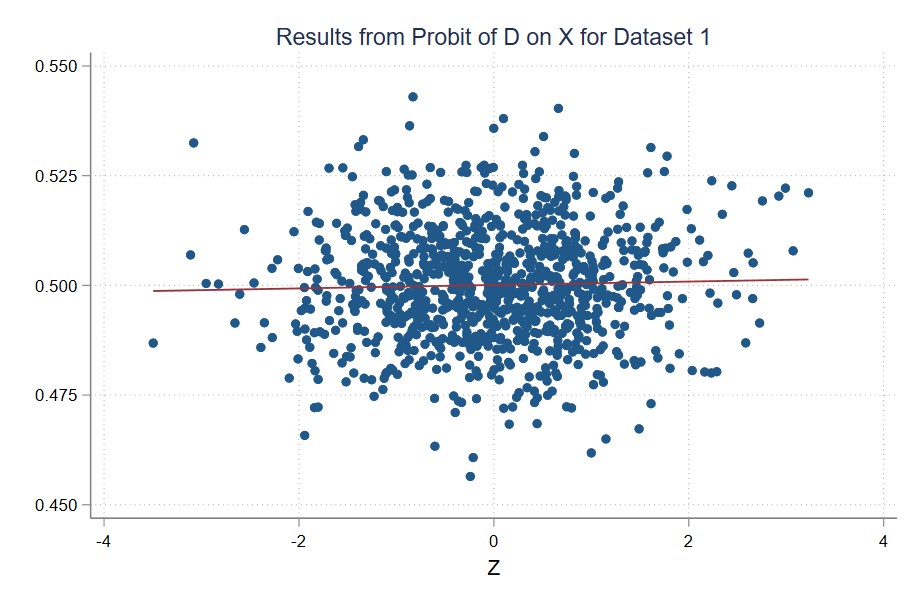
\includegraphics[width=\textwidth]{ps2Heckman/figures/q8_parta_d1.png}
        %\caption{Simulation vs. Analytic}
        %\label{ps1H:q4:fig1a}
    \end{subfigure}
    \begin{subfigure}[b]{0.43\textwidth}
        \centering
        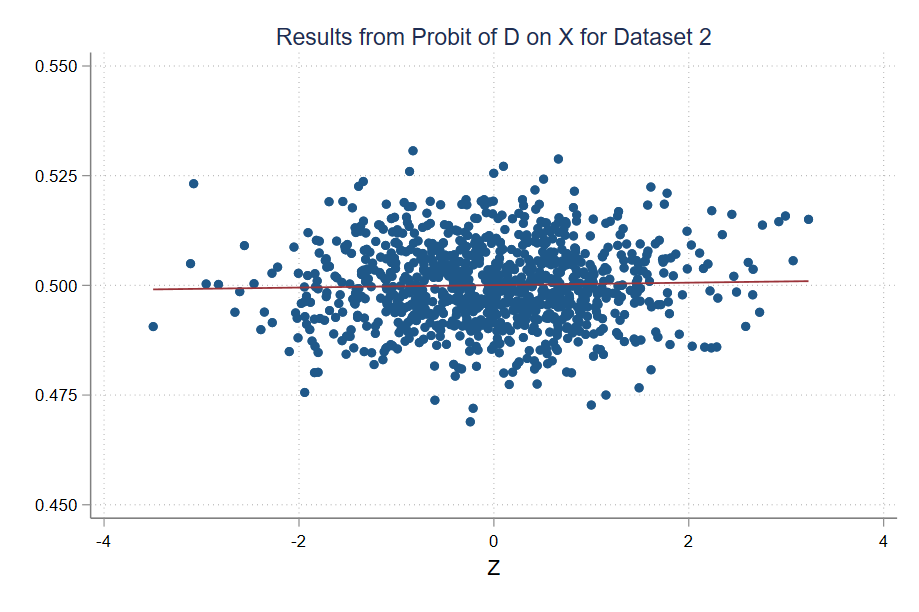
\includegraphics[width=\textwidth]{ps2Heckman/figures/q8_parta_d2.png}
    \end{subfigure}
    \begin{subfigure}[b]{0.43\textwidth}
        \centering
        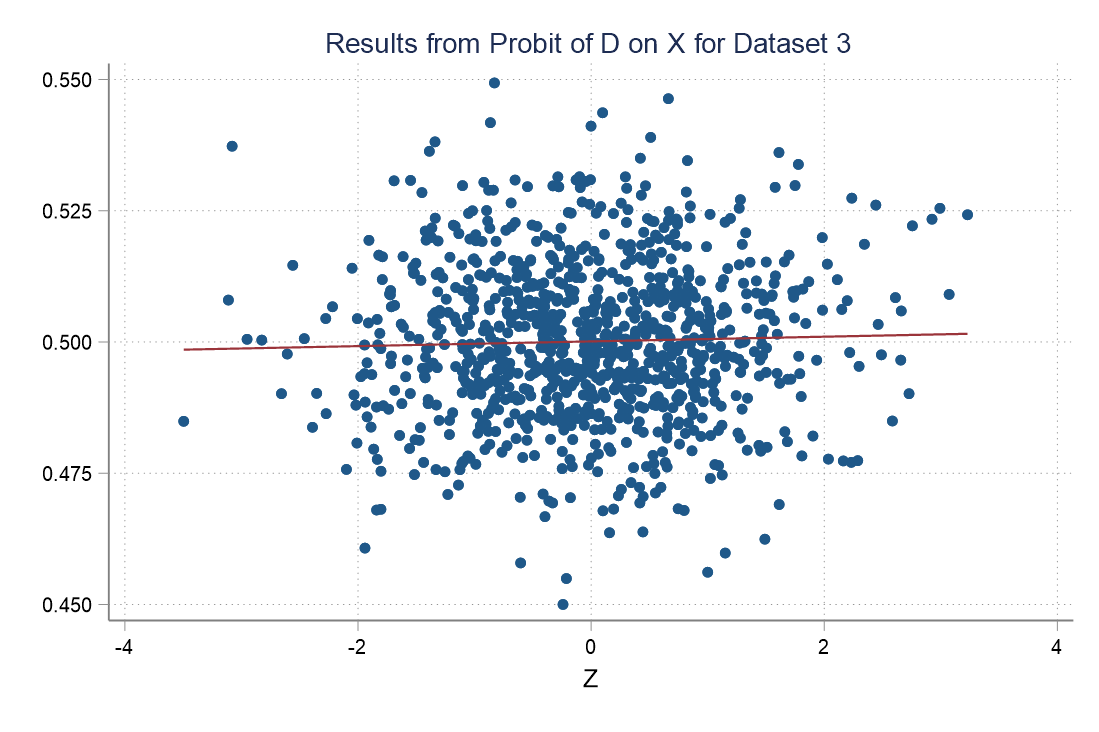
\includegraphics[width=\textwidth]{ps2Heckman/figures/q8_parta_d3.png}
    \end{subfigure}
    \begin{subfigure}[b]{0.43\textwidth}
        \centering
        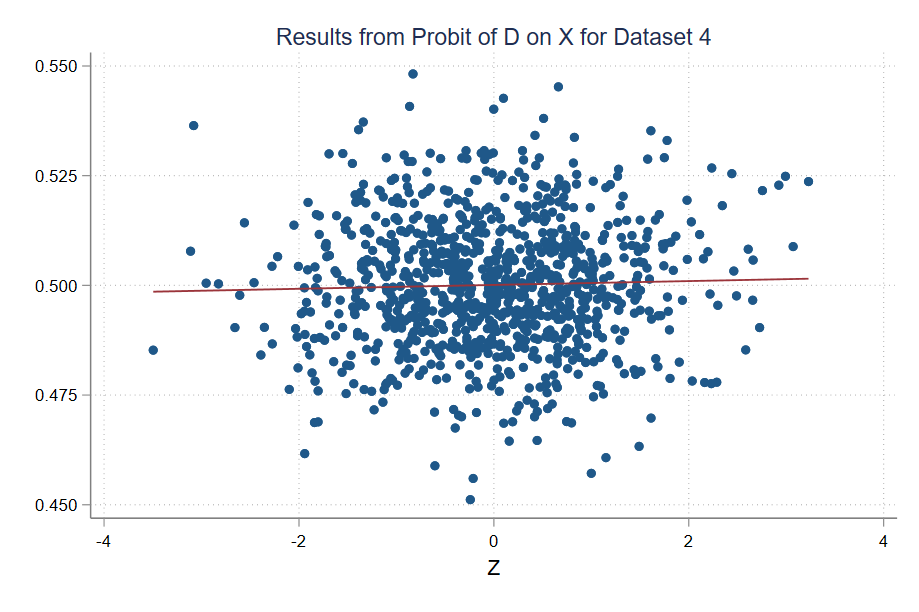
\includegraphics[width=\textwidth]{ps2Heckman/figures/q8_parta_d4.png}
    \end{subfigure}
    \begin{subfigure}[b]{0.43\textwidth}
        \centering
        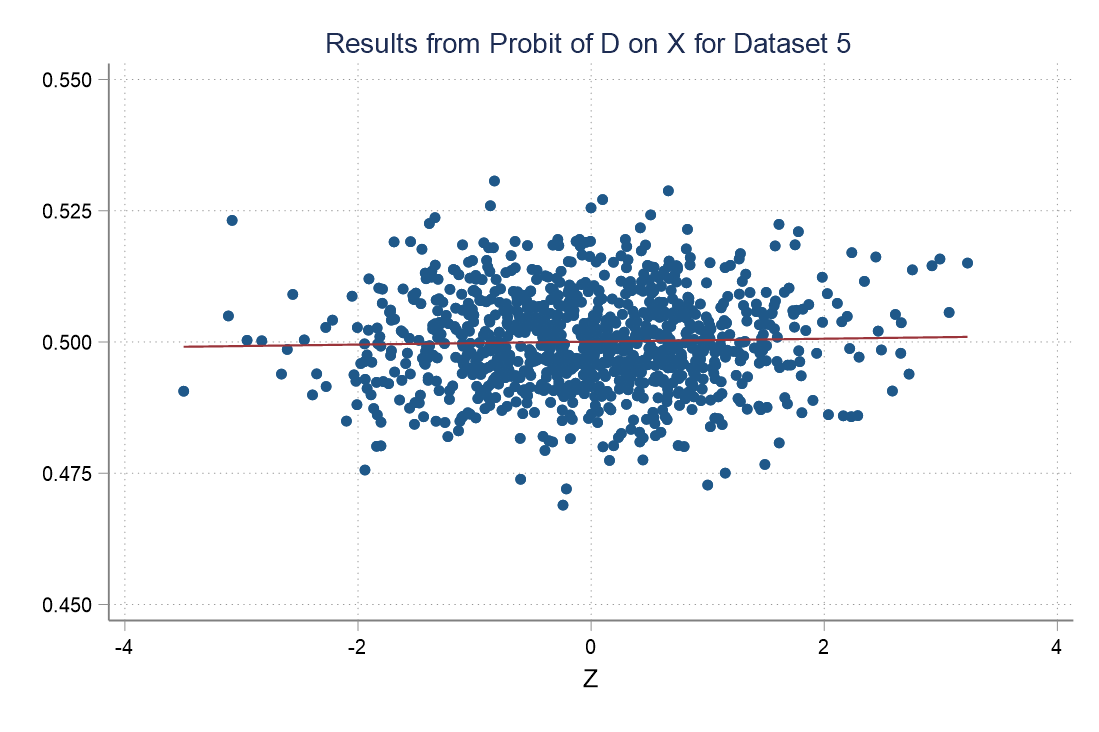
\includegraphics[width=\textwidth]{ps2Heckman/figures/q8_parta_d5.png}
    \end{subfigure}
\end{figure}
\end{solution}

First, let's define what we assume ``subjective treatment effect'' means. Taking the perspective of each individual who chooses whether $D=0$ or $D=0$, we know that this decision takes the form $D=\mathbb{1}\{Y_1-Y_0-C>0\}$. That is, if the subjective benefit $Y_1-Y_0$ are greater than the subjective cost, $C$, the individual chooses state 1 over state 0. So the subjective treatment effect for an individual with $X=x$ and $Z=z$ is:
\begin{align*}
    Y_1 - Y_0 - C &= (\mu_1(x) + U_1) - (\mu_0(x) + U_0) - (\phi(z) + U_c) \\
    &= (\beta_1- \beta_0)x - \beta_C z + U_1 - U_0 - U_c 
\end{align*}
The net benefit to state 1 is $Y_1 - C$ and the net benefit to state 0 is $Y_0$, so the subjective treatment effect is the difference in these two values. Only the first three terms above are observed to the econometrician, whereas the $U_j$s are known to the individual and informs their decision-making process.

\begin{problem}{b}
Use the normal selection correction model to estimate $\beta_{1}$ and $\beta_{0}$. Using your estimates, identify:
\begin{enumerate}[(i)]
    \item $\mathrm{ATE}$
    \item $\mathrm{TT}$
    \item TUT
    \item PRTE (for policy change $Z$ ): Consider the policy changes $Z$ to $Z^{\prime}$ where $Z=0.5$ and $Z^{\prime}=1$ as well as for $Z^{\prime}=-0.5$.
    \item MTE
    \item LATE
\end{enumerate}
(This asks you to use the selection corrected estimates to identify each parameter.)
\end{problem}
\begin{solution}
Please see the attached code for calculations. I use the Heckman two-step correction to estimate the parameters of the Generalized Roy Model, presented below.
\begin{table}[H]
    \centering
    \begin{tabular}{lr r r r r r}
\hline\hline
            &  $\gamma_x$&  $\gamma_w$&   $\beta_1$&   $\beta_0$&    $\rho_1$&    $\rho_0$\\
\hline
1           &       -0.03&        0.05&       -0.08&       -0.02&       -5.81&        0.11\\
2           &       -0.02&       -0.03&       -0.13&       -0.02&       -2.69&        0.17\\
3           &       -0.04&       -0.00&        0.02&        0.02&       -0.21&        0.82\\
4           &       -0.03&        0.05&        0.02&        0.09&       -8.27&       -0.51\\
5           &       -0.02&        0.09&       -0.01&       -0.01&       -2.03&        0.91\\
\hline\hline
\end{tabular}

\end{table}

I then use these parameter estimates to calculate the treatment effects. The table below reports the ATE, ATT, ATUT, PRTE from $z=0.5$ to $z^\prime=1$ and $z^\prime=-0.5$, and the average MTE. Note that these parameters are supposed to be for a \textbf{fixed} $x$, but I calculate them for each observation and then average over the observations' treatment effect. Thus this can be thought of as fixed for $X=0$ since that is the average in the data.
\begin{table}[H]
    \centering
    \begin{center}
\begin{tabular}{lrrrrrr}
\hline \noalign{\smallskip}Dataset & ATE & ATT & ATUT & PRTE1 & PRTE2 & AMTE\\
\noalign{\smallskip}\hline \noalign{\smallskip}1 & 0.000 & 4.732 & -4.722 & -0.002 & -0.000 & 0.008\\
2 & 0.001 & 2.281 & -2.283 & -0.000 & 0.000 & -0.002\\
3 & 0.000 & 0.827 & -0.828 & -0.000 & -0.000 & -0.000\\
4 & 0.000 & 6.197 & -6.184 & -0.003 & -0.000 & 0.010\\
5 & -0.000 & 2.358 & -2.349 & -0.004 & 0.000 & 0.007\\
\noalign{\smallskip}\hline\end{tabular}\\
\end{center}

\end{table}

I then plot these treatment effects against the propensity score $P(Z)$ for each dataset.
\begin{figure}[H]
    \centering
    \caption{$P(D=1|X)$ for each of the five datasets}
    %\label{ps1H:q4:fig1}
    \begin{subfigure}[b]{0.43\textwidth}
        \centering
        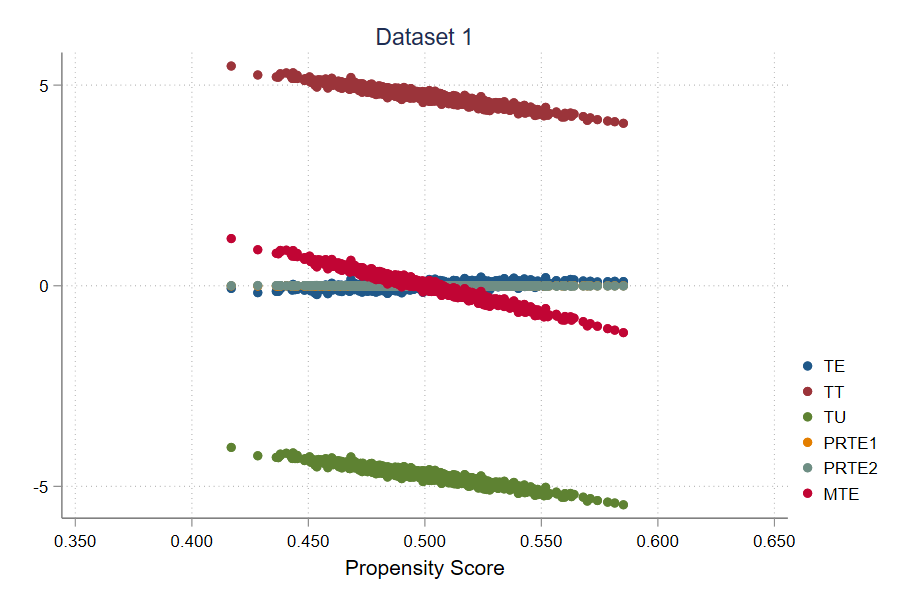
\includegraphics[width=\textwidth]{ps2Heckman/figures/q8_partb_d1_all.png}
        %\caption{Simulation vs. Analytic}
        %\label{ps1H:q4:fig1a}
    \end{subfigure}
    \begin{subfigure}[b]{0.43\textwidth}
        \centering
        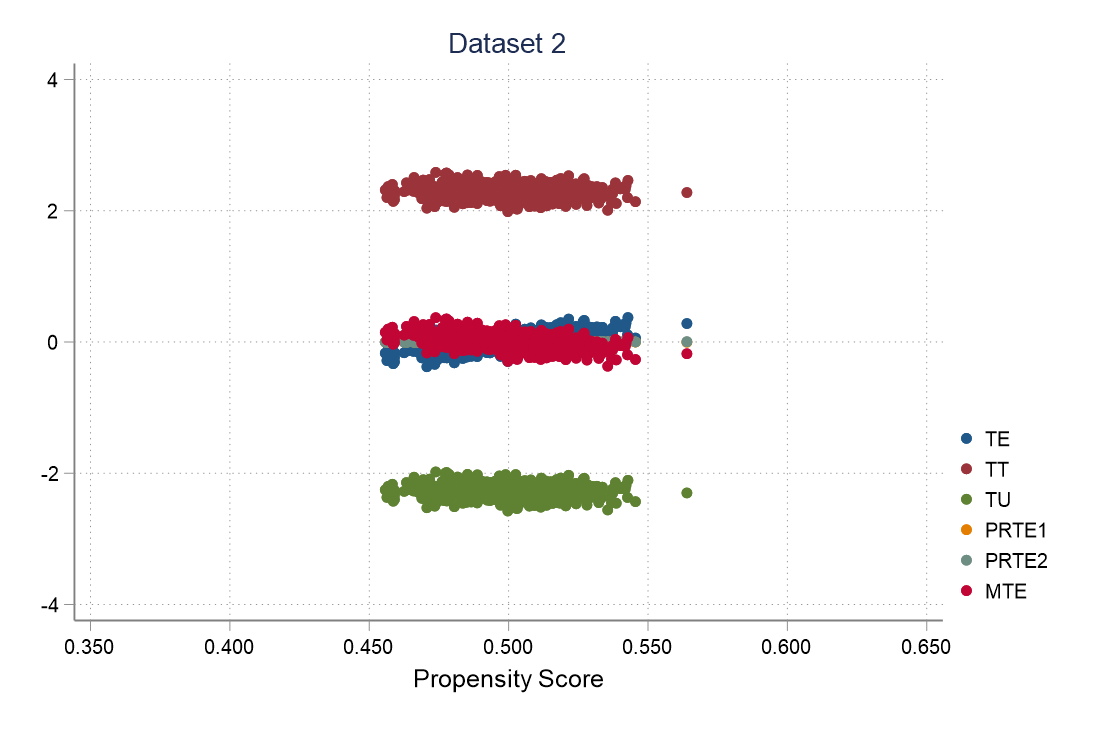
\includegraphics[width=\textwidth]{ps2Heckman/figures/q8_partb_d2_all.png}
    \end{subfigure}
    \begin{subfigure}[b]{0.43\textwidth}
        \centering
        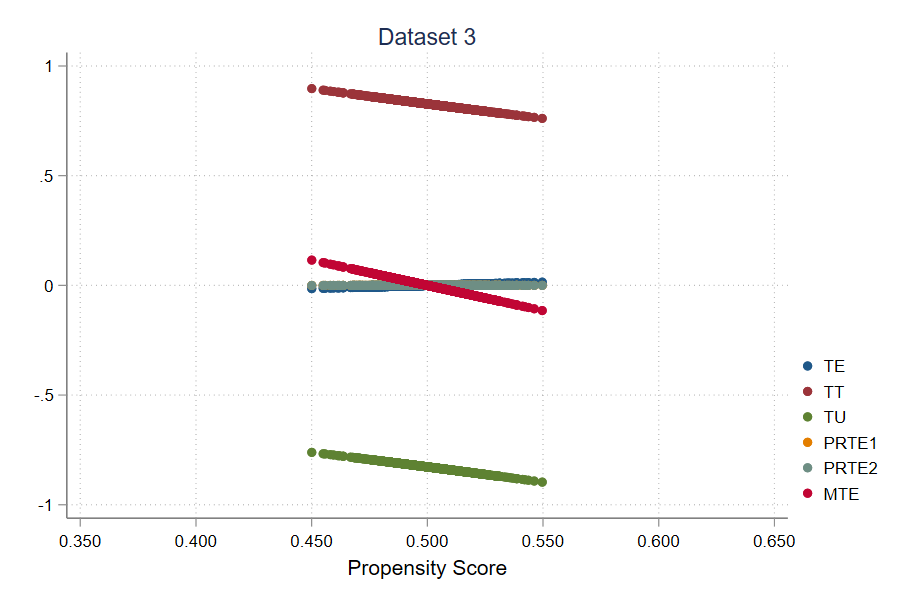
\includegraphics[width=\textwidth]{ps2Heckman/figures/q8_partb_d3_all.png}
    \end{subfigure}
    \begin{subfigure}[b]{0.43\textwidth}
        \centering
        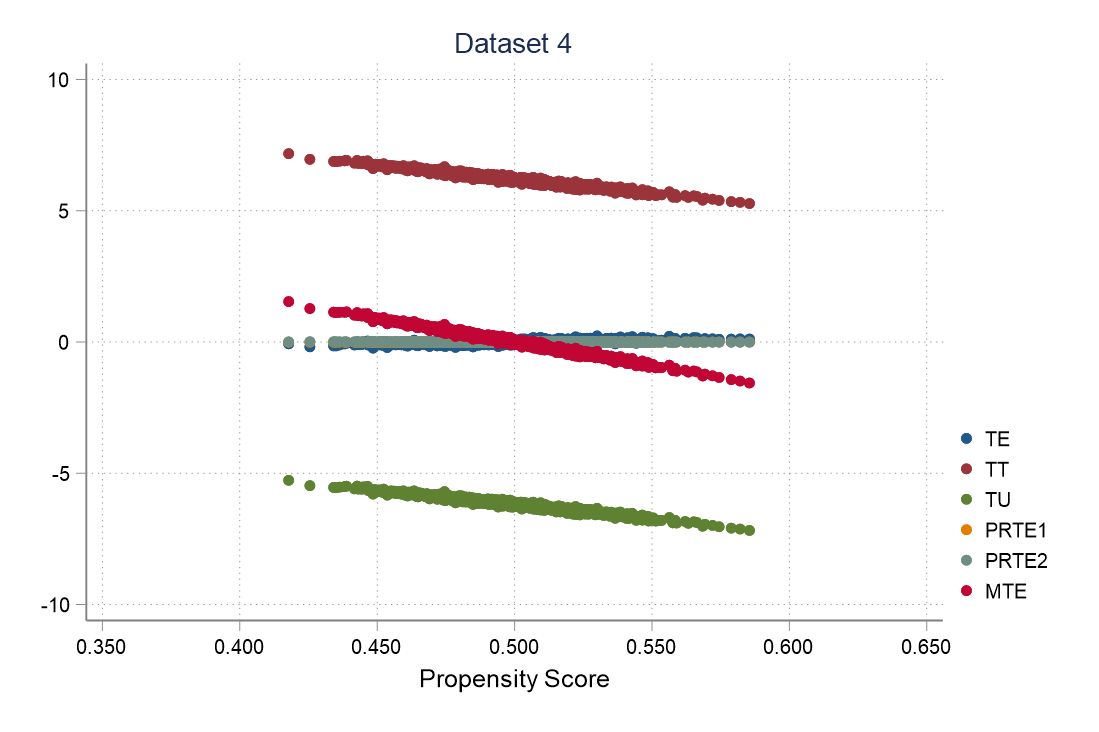
\includegraphics[width=\textwidth]{ps2Heckman/figures/q8_partb_d4_all.png}
    \end{subfigure}
    \begin{subfigure}[b]{0.43\textwidth}
        \centering
        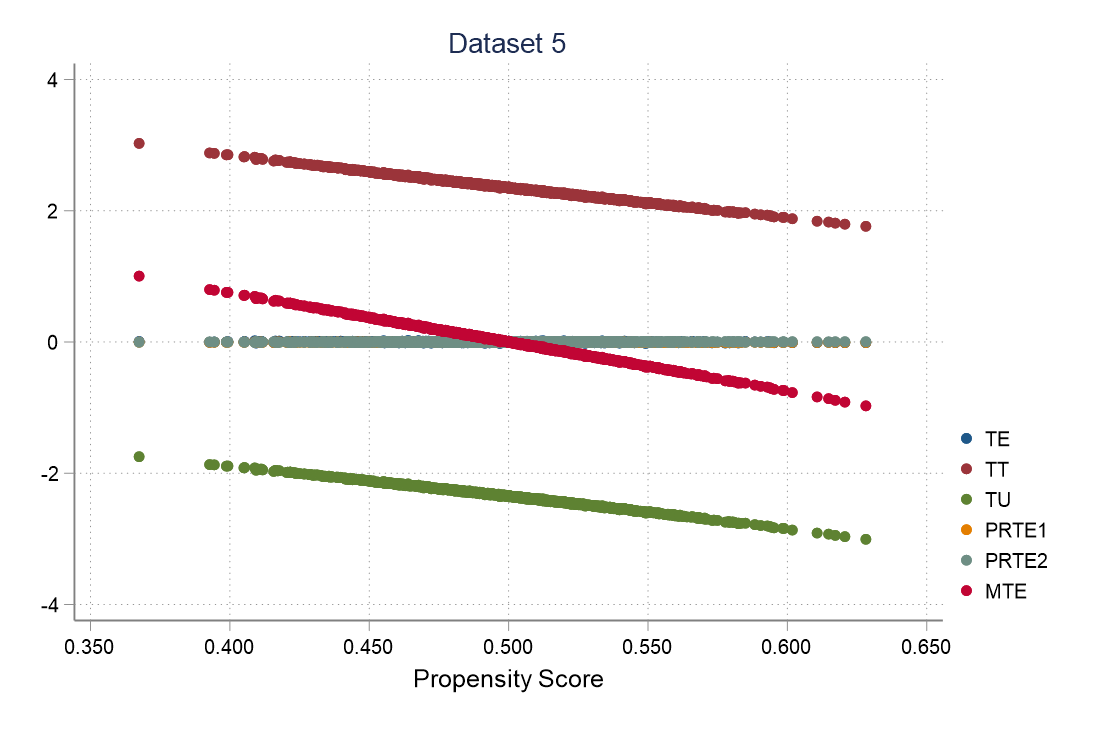
\includegraphics[width=\textwidth]{ps2Heckman/figures/q8_partb_d5_all.png}
    \end{subfigure}
\end{figure}

In this instance, it is unclear what the LATE is since each observation in each dataset has a different $Z$ value. As such, I derive the LATE formula for any instrument shift from $z$ to $z^\prime$. 

Let $\mu_D(X,Z) \equiv \mu_1(X)- \mu_0(X) - \mu_C(Z)$ and $V \equiv - (U_1 - U_0 - U_C)$ such that $D_z = 0 \Leftrightarrow \mu_D(x,z) \leq V $. Then, assuming $\sigma_V=1$:
\begin{align*}
    \operatorname{LATE}(z,z^\prime,x) &= \operatorname{E}[Y_1 - Y_0 \mid D_z = 0, D_{z^\prime}=1,X=x] \\
    &= x(\beta_1 - \beta_0) + E[U_1-U_0 | \mu_D(x,z) \leq V, \mu_D(x,z^\prime) > V, X=x] \\
    &= x(\beta_1 - \beta_0) + E[U_1-U_0 | \mu_D(x,z) \leq V < \mu_D(x,z^\prime) , X=x] \\
    &= x(\beta_1 - \beta_0) + \operatorname{Cov}(U_1-U_0,V) 
    \left( \frac{\phi(\mu_D(x,z))-\phi(\mu_D(x,z^\prime)}{\Phi(\mu_D(x,z^\prime))-\Phi(\mu_D(x,z)} \right)
\end{align*}
Note that if we were given $z$ and $z^\prime$ we could calculate this late since the covariance is $\rho_1 - \rho0$ and the arguments to $\phi$ and $\Phi$ are estimable.
\end{solution}

\begin{problem}{c}
Use the instrument $Z$ to identify the same parameters as in $8(b)$ (i.e., define LATE and address what it identifies). Compare your estimates. Interpret LATE in terms of the MTE.
\end{problem}
\begin{solution}
I have defined the LATE above. The LATE identifies the treatment effect for the individuals whose decision rule changes after $z$ becomes $z^\prime$. As we take the limit of the LATE as the difference between these two instrument values gets closer (or rather, $z^\prime$ approaches $z$), the LATE then becomes the MTE:
\begin{align*}
    \lim _{z^{\prime} \rightarrow z} \operatorname{LATE}\left(z, z^{\prime}, x\right)
    &=x\left(\beta_{1}-\beta_{0}\right)+\operatorname{Cov}\left(U_{1}-U_{0}, V\right) \lim _{z^{\prime} \rightarrow z}\left(\frac{\phi(\mu_D(x,z))-\phi\left(\mu_D(x,z^\prime)\right)}{\Phi\left(\mu_D(x,z^\prime)\right)-\Phi(\mu_D(x,z))}\right) \\
&=x\left(\beta_{1}-\beta_{0}\right)+\operatorname{Cov}\left(U_{1}-U_{0}, v\right)[\mu_D(x,z)] \\
&=\operatorname{MTE}(x,\mu_D(x,z))
\end{align*}
\end{solution}

\begin{problem}{d}
Does LATE identify subjective treatment effects?
\end{problem}
\begin{solution}
No, LATE identifies the average treatment effect for compliers when we shift the instrument and does not capture the cost to an individual of moving from sector 1 to sector 0 (i.e. C).

Perhaps what the question means to ask is if the LATE identified by shifting the instrument from $z$ in the data to $z^\prime=0$, i.e. lowering the cost, is the subjective treatment effect? Still, the LATE does not incorporate the cost to the agent of making said decision, only the gain from treatment. However, LATE does identify the average subjective treatment effect for individuals whose decision of treatment or not changes. In this instance, since we now have $C_{z^\prime}=U_c$, which is mean 0, the subjective treatment effect is $Y_1-Y_0$ and so is the LATE for compliers. Under $z$ in the data, only some observations take up treatment $D_z=1$. With $z^\prime=0$ then the ``compliers'' are those who now take up treatment $D_{z^\prime}=1$. The subjective treatment effect is now the gain that occurs due to treatment when the cost falls to 0, and LATE identifies it for the individuals whose STE is positive under $z^\prime=0$ but was negative under $z$.
\end{solution}

\begin{problem}{e}
Using your estimates from 8(b) and 8(c), compute the gain (or loss) surplus from changing $Z$ to $Z^{\prime}$ where $Z=0.5$ and $Z^{\prime}=1$ as well as for $Z^{\prime}=-0.5$. Write out the formula and compute.
\end{problem}
\begin{solution}
We already calculated the PRTE, which is exactly the gain from changing $z$ to $z^\prime$ for these values. That is, the PRTE is the gross surplus. The net surplus is therefore the gross gain over the cost.

Following Heckman (2010) "Building Bridges", we can write the surplus for two values of $p$ that correspond to $z$ and $z^\prime$ as:
\begin{align*}
    S(p_2) - S(p_1) &= E[Y_1-Y_0| p_1 \leq U_D \leq p_2] \times P(p_1 \leq U_D \leq p_2) \\
    &= E[Y_1-Y_0| p_1 \leq U_D \leq p_2] (p_2-p_1) \\
    &= \int_{p_1}^{p_2} \operatorname{MTE}(u_D) \operatorname{d} u_D
\end{align*}
Where we note that if we divided this value by $p_2-p_1$ then this would be the LATE. Using our Generalized Roy Model setup, we can calculate the surplus above as:
\begin{align*}
    S(p_2) - S(p_1) &= \int_{p_1}^{p_2} \operatorname{MTE}(u_D) \operatorname{d} u_D \\
    &= \int_{F_V^{-1}(p_1)}^{F_V^{-1}(p_2)} \operatorname{MTE}(v) f_V(v) \operatorname{d} v \\
    &= \int_{F_V^{-1}(p_1)}^{F_V^{-1}(p_2)} E[Y_1-Y_0 | F_V(V)=V] f_V(v) \operatorname{d} v \\
    &= x(\beta_1-\beta_0) \int_{F_V^{-1}(p_1)}^{F_V^{-1}(p_2)}f_V(v)\operatorname{d} v  + 
    \int_{F_V^{-1}(p_1)}^{F_V^{-1}(p_2)} E[U_1 - U_0 | F_V(V)=V] f_V(v) \operatorname{d} v \\
    &= x(\beta_1-\beta_0) (p_2-p_1)  + 
    \int_{F_V^{-1}(p_1)}^{F_V^{-1}(p_2)}\operatorname{Cov}(U_1 - U_0,V) E[V | F_V(V)=V] f_V(v) \operatorname{d} v \\
    &= x(\beta_1-\beta_0) (p_2-p_1)  + 
    \int_{F_V^{-1}(p_1)}^{F_V^{-1}(p_2)}\operatorname{Cov}(U_1 - U_0,V) v f_V(v) \operatorname{d} v \\
    &= x(\beta_1-\beta_0) (p_2-p_1) + \operatorname{Cov}(U_1 - U_0,V) (f_V(F_V^{-1}(p_1)) - f_V(F_V^{-1}(p_2))  \\
    &= x(\beta_1-\beta_0) (p_2-p_1) + \operatorname{Cov}(U_1 - U_0,V) (\phi(\Phi^{-1}(p_1)) - \phi(\Phi^{-1}(p_2))  \\
\end{align*}
Where we've used the fact that $f_V(\cdot)=\phi(\cdot)$ and properties of the normal distribution.

Since we have the $\beta$s and $\rho$s from before, all we need to do is calculate $p_1$ and $p_2$ using the $\gamma$s from earlier. Using the mean value of $x$ for each dataset, the results for the surplus are:
%\begin{table}[H]
%    \centering
%    \begin{tabular}{lrr}
\hline \noalign{\smallskip}Dataset & Surplus 1 & Surplus 2\\
\noalign{\smallskip}\hline \noalign{\smallskip}1 & -2.20 & -2.20\\
2 & -1.05 & -1.05\\
3 & -0.38 & -0.38\\
4 & -2.89 & -2.88\\
5 & -1.10 & -1.10\\
\noalign{\smallskip}\hline\end{tabular}\\

%\end{table}


\end{solution}







\end{document}
